\documentclass[11pt,a4paper]{ctexart}

% Page geometry
\usepackage[top=2.5cm, bottom=2.5cm, left=2.5cm, right=2.5cm]{geometry}

% Math and physics
\usepackage{amsmath,amssymb}
\usepackage{physics}

% Tables
\usepackage{booktabs, longtable, array}

% Graphics
\usepackage{graphicx, float, tikz}
\usetikzlibrary{arrows.meta, positioning, shapes, calc, fit}

% Hyperlinks
\usepackage{hyperref}
\hypersetup{colorlinks=true, linkcolor=blue, citecolor=blue, urlcolor=blue}

% Code
\usepackage{listings}
\lstset{
  basicstyle=\ttfamily\small,
  breaklines=true,
  frame=single,
  language=Python,
  tabsize=2,
  showstringspaces=false,
}

% Color boxes
\usepackage{xcolor, tcolorbox}
\newtcolorbox{designbox}{colback=blue!3, colframe=blue!50!black,
    title=\textbf{设计决策}, fonttitle=\bfseries}
\newtcolorbox{warnbox}{colback=red!3, colframe=red!50!black,
    title=\textbf{注意事项}, fonttitle=\bfseries}
\newtcolorbox{paramtable}{colback=gray!3, colframe=gray!50!black,
    title=\textbf{参数表}, fonttitle=\bfseries}

\title{Q 函数反演：工程实施方案\\
    \textnormal{\large ——从理论基础到模块化数值程序}}
\author{Q-Inversion Project}
\date{2026-07-24 · v1.0}

\begin{document}

\maketitle

\begin{abstract}
本文档将 \texttt{Q函数重建\_v3\_完整论证.pdf} 中的理论推导转化为可实施的工程方案。
核心算法是\textbf{模糊 Radon 变换的 Fourier 切片定理}：对每个延迟 $\tau$ 做动量方向
1D FFT，在 2D Fourier 空间中采样 $\hat{Q}(\boldsymbol{\xi})$，去模糊后经 2D IFFT
重建 $Q(\boldsymbol{\alpha})$。本文档定义模块架构、参数体系（namelist）、数据格式、
计算流程、采样策略和验证方案，参考 v5.1-release 的工程风格：模块化、参数分离、
单文件可运行、渐进复杂度。
\end{abstract}

\tableofcontents
\newpage

% ======================================================================
\section{项目定位与目标}

\subsection{与 v5.1-release 的关系}

v5.1-release 是\textbf{正向求解器}：
\[
Q(\alpha) \;\xrightarrow{\text{采样}}\; \{\alpha_i, w_i\} \;\xrightarrow{\text{TDSE}}\;
\{A_i(k,\tau)\} \;\xrightarrow{\text{合成}}\; P(k,\tau)
\]

本子项目是\textbf{逆向求解器}：
\[
P(k,\tau) \;\xrightarrow{\text{反演}}\; Q(\alpha)
\]

两者共享：
\begin{itemize}
    \item 物理参数定义（$\kappa$, $\sigma_k$, $k_0$, $\omega$, $f(\tau)$）
    \item 数据格式（$P(k,\tau)$ 表格）
    \item 可视化工具链
\end{itemize}

\subsection{设计原则}

\begin{enumerate}
    \item \textbf{单文件可运行}：核心反演由一个 Python 脚本完成，依赖仅限 numpy/scipy
    \item \textbf{参数分离}：所有物理/数值参数通过 namelist 风格的配置文件传入
    \item \textbf{渐进复杂度}：先从对角近似 + 均匀 $\tau$ 网格起步，逐步加入正则化和非均匀采样
    \item \textbf{可验证性}：内置 closed-loop 测试（已知 Q → 模拟 P → 反演 → 对比）
\end{enumerate}

% ======================================================================
\section{理论基础的精简复述}

\subsection{正向模型（对角近似）}

\begin{equation}\label{eq:forward}
    P(k;\tau) = \iint d^2\alpha \; Q(\boldsymbol{\alpha}) \;
    \frac{J(k,\tau)}{\sqrt{2\pi}\,\sigma_k} \,
    \exp\!\left[-\frac{\bigl(k - k_0 + \boldsymbol{\kappa}(\tau)\!\cdot\!\boldsymbol{\alpha}\bigr)^2}
    {2\sigma_k^2}\right]
\end{equation}

定义归一化谱 $\tilde{P}(k;\tau) \equiv P(k;\tau) / J(k,\tau)$（$J$ 缓变时可先取常数），
则正问题为 Gaussian 核卷积。

\subsection{Fourier 切片定理（精确）}

对 $\tilde{P}$ 做 $k$ 方向 1D Fourier 变换：
\begin{equation}\label{eq:slice}
    \boxed{\tilde{P}(\omega_k,\tau)
    = e^{-i\omega_k k_0} \; e^{-\omega_k^2\sigma_k^2/2} \;
    \hat{Q}\bigl(\omega_k\,\boldsymbol{\kappa}(\tau)\bigr)}
\end{equation}

其中 $\boldsymbol{\kappa}(\tau) = \kappa f(\tau)(\sin\omega\tau,\;\cos\omega\tau)^T$。

\textbf{物理解释：} 固定 $\tau$，$\tilde{P}(\omega_k,\tau)$ 给出 $\hat{Q}$ 在
$\boldsymbol{\xi} = \omega_k\boldsymbol{\kappa}(\tau)$ 处的值——即沿方向 $\boldsymbol{\kappa}(\tau)$、
距原点 $\omega_k\kappa f(\tau)$ 的采样点。

\subsection{反演步骤（5 步）}

\begin{enumerate}
    \item \textbf{1D FFT}：对每个 $\tau$，沿 $k$ 方向 FFT → $\tilde{P}(\omega_k,\tau)$
    \item \textbf{去模糊}：$\hat{Q}(\omega_k\boldsymbol{\kappa}(\tau))
        = e^{+i\omega_k k_0}\, e^{+\omega_k^2\sigma_k^2/2}\,
        \tilde{P}(\omega_k,\tau)$
    \item \textbf{截断}：在 $|\omega_k| > \omega_k^{\max}$ 处截止，抑制噪声放大
    \item \textbf{2D 网格化}：将径向采样点 $(\omega_k,\tau)$ 映射到笛卡尔
        $(\xi_R,\xi_I)$，插值到均匀网格
    \item \textbf{2D IFFT}：逆变换 → $Q(\boldsymbol{\alpha})$
\end{enumerate}

% ======================================================================
\section{模块架构}

\subsection{总体结构}

\begin{center}
\begin{tikzpicture}[
    node distance=0.8cm,
    box/.style={rectangle, draw, rounded corners, minimum width=3.5cm, minimum height=0.7cm, align=center, font=\small},
    data/.style={rectangle, draw, fill=gray!10, minimum width=3cm, minimum height=0.6cm, align=center, font=\small},
    arrow/.style={-{Stealth}, thick}
]
    % Top level
    \node[box, fill=blue!10] (driver) {\texttt{invert\_q.py}\\主入口};

    % Input
    \node[data, above=of driver] (pdata) {$P(k,\tau)$ 实测数据};
    \node[data, left=1.5cm of driver] (config) {\texttt{qinv.nml}\\配置文件};
    \node[data, right=1.5cm of driver] (forward) {正向模型参数\\（核函数）};

    % Processing modules
    \node[box, below left=1cm and -0.5cm of driver, fill=green!8] (fft) {\texttt{transform}\\1D FFT + 去模糊};
    \node[box, below right=1cm and -0.5cm of driver, fill=green!8] (grid) {\texttt{gridding}\\Fourier 空间网格化};
    \node[box, below=of driver, fill=green!8] (deblur) {\texttt{deblur}\\截断 + 正则化};
    \node[box, below=0.8cm of fft, fill=green!8] (ifft) {\texttt{reconstruct}\\2D IFFT → Q};

    % Output
    \node[data, below=1cm of ifft] (qout) {$Q(\alpha)$ 网格 + 图};

    % Arrows
    \draw[arrow] (config) -- (driver);
    \draw[arrow] (pdata) -- (driver);
    \draw[arrow] (forward) -- (driver);
    \draw[arrow] (driver) -- (fft);
    \draw[arrow] (fft) -- (deblur);
    \draw[arrow] (deblur) -- (grid);
    \draw[arrow] (grid) -- (ifft);
    \draw[arrow] (ifft) -- (qout);

    % Phase labels
    \node[font=\small\bfseries, right=0.3cm of fft] {Phase 1};
    \node[font=\small\bfseries, right=0.3cm of deblur] {Phase 2};
    \node[font=\small\bfseries, right=0.3cm of grid] {Phase 3};
    \node[font=\small\bfseries, right=0.3cm of ifft] {Phase 4};

\end{tikzpicture}
\end{center}

\subsection{模块职责}

\begin{table}[H]
\centering
\caption{模块职责与接口}
\begin{tabular}{p{2.5cm}p{3cm}p{4.5cm}p{3cm}}
\toprule
\textbf{模块} & \textbf{文件} & \textbf{职责} & \textbf{输入/输出} \\
\midrule
\texttt{config} & \texttt{config.py} & 读取/校验 namelist 风格参数 & IN: \texttt{.nml} 文件
    OUT: \texttt{QInvConfig} 对象 \\
\midrule
\texttt{io\_data} & \texttt{io\_data.py} & 读写 $P(k,\tau)$ 和 $Q(\alpha)$ 数据文件
    & IN/OUT: ASCII 表格 \\
\midrule
\texttt{forward\_model} & \texttt{forward\_model.py} & 正向核函数的 J, $\kappa(\tau)$,
    $\sigma_k$, $k_0$ & IN: config, $\tau$ 数组
    OUT: kernel params \\
\midrule
\texttt{transform} & \texttt{transform.py} & 1D FFT + 去模糊 + 截断
    & IN: $\tilde{P}(k,\tau)$
    OUT: $\hat{Q}$ 径向采样点 \\
\midrule
\texttt{gridding} & \texttt{gridding.py} & 径向 → 笛卡尔插值
    & IN: $(\xi_R,\xi_I, \hat{Q})$ 散点
    OUT: $\hat{Q}$ 笛卡尔网格 \\
\midrule
\texttt{reconstruct} & \texttt{reconstruct.py} & 2D IFFT → $Q(\alpha)$
    & IN: $\hat{Q}$ 网格
    OUT: $Q(\alpha_R,\alpha_I)$ 网格 \\
\midrule
\texttt{regularize} & \texttt{regularize.py} & Tikhonov/TV/MaxEnt 正则化
    & IN: 带噪声的 $\hat{Q}$
    OUT: 正则化后的 $\hat{Q}$ \\
\midrule
\texttt{diagnostics} & \texttt{diagnostics.py} & 残差、分辨率估计、Fourier 覆盖率
    & IN: 反演结果
    OUT: 诊断报告 \\
\midrule
\texttt{invert\_q} & \texttt{invert\_q.py} & 主入口：组装流水线 + CLI
    & IN: cli args + config
    OUT: $Q(\alpha)$ 文件 + 图 \\
\bottomrule
\end{tabular}
\end{table}

\begin{designbox}
\textbf{语言选择：Python 优先。} 反演计算以 FFT + 插值为主，Python + numpy/scipy 足够。
若后续需要与 v5.1 的 Fortran 正向模型紧密耦合（如迭代反演中频繁调用 TDSE），可将正向模型
封装为 Python 可调用的子进程或 f2py 模块。正则化中的最优化部分若成为瓶颈，可下沉到
Cython/numba。
\end{designbox}

% ======================================================================
\section{参数体系}

\subsection{参数分类}

参数分为三类，沿用 v5.1 的 namelist 分组风格：

\begin{table}[H]
\centering
\caption{参数分组}
\begin{tabular}{p{2.5cm}p{3cm}p{7cm}}
\toprule
\textbf{组名} & \textbf{语义} & \textbf{内容} \\
\midrule
\texttt{\&physics} & 物理参数 & 激光参数、原子参数、核函数参数 \\
\texttt{\&numerics} & 数值参数 & FFT 点数、网格分辨率、截断/正则化参数 \\
\texttt{\&io} & I/O 参数 & 输入/输出路径、格式选择 \\
\bottomrule
\end{tabular}
\end{table}

\subsection{\texttt{\&physics} — 物理参数}

\begin{paramtable}
\begin{longtable}{p{2.8cm}p{1.5cm}p{2cm}p{5.5cm}}
\toprule
\textbf{参数} & \textbf{类型} & \textbf{默认值} & \textbf{说明} \\
\midrule
\texttt{nir\_omega}    & real & 0.057  & NIR 光子能量 (a.u.), 800 nm → 0.057 \\
\texttt{nir\_e0}       & real & 0.04   & NIR 单光子场幅 $\mathcal{E}_N$ (a.u.) \\
\texttt{kappa}         & real & 计算值  & 有效 streaking 振幅 $\kappa = 2\mathcal{E}_N/\omega$；若 $>0$ 则覆盖自动计算 \\
\texttt{k0}            & real & 1.0    & 无场光电子动量 $k_0 = \sqrt{2(\Omega_{\mathrm{XUV}} - I_p)}$ (a.u.) \\
\texttt{sigma\_k}      & real & 0.1    & 动量展宽 $\sigma_k$ (a.u.)，量级 $\sim 1/\tau_X$ \\
\texttt{ip}            & real & 0.5    & 电离势 (a.u.), 氢原子 $I_p = 0.5$ \\
\texttt{use\_diagonal} & bool & T & 是否使用对角近似（忽略 $P_{\text{off}}$） \\
\bottomrule
\end{longtable}
\end{paramtable}

\begin{designbox}
\textbf{参数推导规则：} $\kappa$ 默认由 $\kappa = 2\mathcal{E}_N / \omega$ 自动计算；
$\sigma_k$ 默认由 $\sigma_k \approx 1/\tau_X$ 估计（$\tau_X$ 为 XUV 脉宽）。
用户可直接覆盖以适配非标准场景。
\end{designbox}

\subsection{\texttt{\&numerics} — 数值参数}

\begin{paramtable}
\begin{longtable}{p{2.8cm}p{1.5cm}p{2cm}p{5.5cm}}
\toprule
\textbf{参数} & \textbf{类型} & \textbf{默认值} & \textbf{说明} \\
\midrule
\texttt{n\_k}           & int  & 256    & $P(k,\tau)$ 中 $k$ 方向的点数；同时是 1D FFT 尺寸 \\
\texttt{n\_tau}         & int  & 64     & $\tau$ 延迟采样数（每 NIR 周期） \\
\texttt{n\_tau\_cycles} & int  & 1      & $\tau$ 扫描覆盖的 NIR 周期数 \\
\texttt{n\_xi}          & int  & 128    & Fourier 空间 $(\xi_R,\xi_I)$ 的笛卡尔网格尺寸（单边） \\
\texttt{n\_alpha}       & int  & 128    & 实空间 $(\alpha_R,\alpha_I)$ 的网格尺寸（单边） \\
\texttt{omega\_k\_max}  & real & 自动   & 截断频率 (a.u.)；默认由 SNR 公式自动计算 \\
\texttt{snr\_p}         & real & 100.0  & $P(k,\tau)$ 的信噪比估计（用于截断频率计算） \\
\texttt{snr\_q\_target} & real & 10.0   & 目标 $Q$ 的信噪比（用于截断频率计算） \\
\texttt{interp\_method} & str  & 'rbf'  & 网格化插值方法：\texttt{'linear'}, \texttt{'rbf'}, \texttt{'nearest'} \\
\texttt{regularize}     & str  & 'cutoff' & 正则化策略：\texttt{'cutoff'}, \texttt{'tikhonov'}, \texttt{'tv'}, \texttt{'none'} \\
\texttt{tikhonov\_lambda}& real& 0.01   & Tikhonov 正则化参数（仅 \texttt{regularize='tikhonov'}） \\
\bottomrule
\end{longtable}
\end{paramtable}

\subsection{\texttt{\&io} — I/O 参数}

\begin{paramtable}
\begin{longtable}{p{2.8cm}p{1.5cm}p{2cm}p{5.5cm}}
\toprule
\textbf{参数} & \textbf{类型} & \textbf{默认值} & \textbf{说明} \\
\midrule
\texttt{input\_file}      & str & 必填 & 输入 $P(k,\tau)$ 数据文件路径 \\
\texttt{input\_format}    & str & 'v5.1' & 输入格式：\texttt{'v5.1'}（v5.1 9列格式）,
                                          \texttt{'compact'}（矩阵格式） \\
\texttt{output\_dir}      & str & './output' & 输出目录 \\
\texttt{output\_prefix}   & str & 'qinv' & 输出文件前缀 \\
\texttt{plot}             & bool& T & 是否自动生成可视化 \\
\bottomrule
\end{longtable}
\end{paramtable}

\subsection{Namelist 文件示例}

\begin{lstlisting}[language=Python, caption=典型的 \texttt{qinv.nml} 配置文件, label=lst:namelist]
&physics
  nir_omega = 0.057
  nir_e0 = 0.04
  k0 = 1.0
  sigma_k = 0.08
  ip = 0.5
  use_diagonal = .true.
/

&numerics
  n_k = 256
  n_tau = 64
  n_tau_cycles = 1
  n_xi = 128
  n_alpha = 128
  snr_p = 100.0
  interp_method = 'rbf'
  regularize = 'cutoff'
/

&io
  input_file = '../v5.1-release/projects/my_run/output_20260101_120000/prj_tau_k_summary.dat'
  input_format = 'v5.1'
  output_dir = './output'
  output_prefix = 'bsv_r3'
  plot = .true.
/
\end{lstlisting}

% ======================================================================
\section{数据格式规范}

\subsection{输入：$P(k,\tau)$ 数据}

\textbf{格式 A（v5.1 兼容）}：直接读取 v5.1 的 \texttt{prj\_probability\_tau.dat} 或
\texttt{prj\_tau\_k\_summary.dat}。前者是 9 列格式，后者是 $k$ 方向的角向平均值。

\begin{lstlisting}[caption=v5.1 probability\_tau.dat 格式（9列）, label=lst:input]
# itau  tau(au)  ik  k(au)  itheta  theta(rad)  iphi  phi(rad)  probability
      1  0.00000   1  0.020       1    0.00000     1    0.00000    1.234e-08
      1  0.00000   2  0.035       1    0.00000     1    0.00000    2.456e-08
      ...
\end{lstlisting}

预处理步骤：按 $(\tau, k)$ 分组，对 $\theta,\phi$ 加权求和得到 $P(k,\tau)$。

\textbf{格式 B（紧凑矩阵）}：一个 $N_\tau \times N_k$ 的 ASCII 矩阵，第一行为 $k$ 网格，
第一列为 $\tau$ 网格。

\begin{designbox}
\textbf{首选格式 A（v5.1 兼容）。} 设计阶段的测试数据完全来自 v5.1 模拟输出，
直接兼容可减少格式转换环节。格式 B 作为后续实验数据导入的备选。
\end{designbox}

\subsection{输出：$Q(\alpha)$ 数据}

\begin{lstlisting}[caption=Q 函数输出格式, label=lst:output]
# Q-function reconstruction
# alpha_R_min  alpha_R_max  n_alpha_R
# alpha_I_min  alpha_I_max  n_alpha_I
# Column 1: alpha_R, Column 2: alpha_I, Column 3: Q(alpha_R, alpha_I)
  -8.000  -8.000  1.234e-06
  -8.000  -7.875  2.345e-06
  ...
\end{lstlisting}

网格范围由 $\xi_{\max} \approx \omega_k^{\max} \cdot \kappa_{\max}$ 和
$\Delta\alpha = 2\pi / (2\xi_{\max})$ 自动确定。

% ======================================================================
\section{计算流程详解}

\subsection{Phase 0：数据预处理}

\begin{enumerate}
    \item 读取 $P(k,\tau)$ 数据（v5.1 9列格式）
    \item 对 $\theta,\phi$ 加权求和：$P(k_m,\tau_j) = \sum_{\theta,\phi}
        P(k_m,\theta,\phi;\tau_j)\,k_m^2\sin\theta\,\Delta\theta\Delta\phi$
    \item 构建均匀 $k$ 网格：$k_m = k_{\min} + m\Delta k,\; m=0,\ldots,N_k-1$
    （若原始数据非均匀，先插值）
    \item 归一化 $J$ 校准（首版取 $J=1$，后续从参考 $Q$ 或独立测量标定）
    \item $\tilde{P}(k_m,\tau_j) = P(k_m,\tau_j) / J(k_m,\tau_j)$
\end{enumerate}

\subsection{Phase 1：1D FFT + 去模糊}

对每个 $\tau_j$（$j=1,\ldots,N_\tau$）：

\begin{enumerate}
    \item 沿 $k$ 方向做 $N_k$ 点 FFT：
        $\tilde{P}_j[\ell] = \sum_{m=0}^{N_k-1} \tilde{P}(k_m,\tau_j)\,
        e^{-i 2\pi \ell m / N_k},\quad \ell = 0,\ldots,N_k-1$
    \item 频率轴：$\omega_k[\ell] = 2\pi\ell/(N_k\Delta k)$（正频率）
        和 $\omega_k[\ell] = 2\pi(\ell - N_k)/(N_k\Delta k)$（负频率）
    \item 去模糊：对每个 $\ell$，
        $\hat{Q}_j[\ell] = e^{+i\omega_k[\ell] k_0}\,
        e^{+\omega_k[\ell]^2\sigma_k^2/2}\, \tilde{P}_j[\ell]$
    \item 截断：将 $|\omega_k[\ell]| > \omega_k^{\max}$ 的 $\hat{Q}_j[\ell]$ 置零
    \item 映射到 2D Fourier 坐标：
        $\boldsymbol{\xi}_{j\ell} = \omega_k[\ell] \cdot \boldsymbol{\kappa}(\tau_j)$
\end{enumerate}

\textbf{计算量：} $N_\tau$ 次 $N_k$ 点 FFT $\approx O(N_\tau N_k \log N_k)$，远小于正向 TDSE。

\subsection{Phase 2：Fourier 空间网格化}

将散点 $\{(\xi_R^{(s)}, \xi_I^{(s)}, \hat{Q}^{(s)})\}$ 插值到 $N_\xi \times N_\xi$ 笛卡尔网格：

\begin{enumerate}
    \item 确定网格范围：$\xi_{\max} = \omega_k^{\max} \cdot \kappa \cdot
        \max_\tau f(\tau)$
    \item 构建网格：$\xi_R[p] = -\xi_{\max} + p\Delta\xi,\;
        \xi_I[q] = -\xi_{\max} + q\Delta\xi,\;
        \Delta\xi = 2\xi_{\max}/(N_\xi-1)$
    \item 插值（默认 RBF thin-plate spline；小数据集用 linear）
    \item 对未覆盖区域填零（无数据即假设 $\hat{Q}=0$）
\end{enumerate}

\begin{warnbox}
\textbf{插值方法选择：} RBF 对非均匀散点效果好但计算量 $O(N_{\text{samples}}^2)$。
若 $N_\tau \times N_k$ 很大（$>10^5$ 散点），先用 nearest-neighbor 做初步网格化，
再用 Gaussian 平滑。
\end{warnbox}

\subsection{Phase 3：正则化（可选）}

截断本身就是最简单的正则化。若截断后仍有振荡伪影，追加：

\begin{itemize}
    \item \textbf{Tikhonov：} $\hat{Q}_{\text{reg}} = \hat{Q} / (1 + \lambda|\boldsymbol{\xi}|^2)$
        ——相当于对高频分量阻尼
    \item \textbf{Total Variation：} 对 $Q(\alpha)$ 做 TV 去噪（适用于分段常数 Q）
    \item \textbf{最大熵：} 适用于正定、平滑的 Q 分布
\end{itemize}

\subsection{Phase 4：2D IFFT → $Q(\alpha)$}

\begin{equation}
    Q(\alpha_R[p], \alpha_I[q]) = \frac{1}{(2\pi)^2} \sum_{u,v}
    \hat{Q}_{\text{grid}}[u,v]\,
    e^{-i(\xi_R[u]\alpha_R[p] + \xi_I[v]\alpha_I[q])}\,
    \Delta\xi_R\Delta\xi_I
\end{equation}

实际使用 numpy 的 \texttt{ifft2}（需注意归一化和象限顺序）。

\subsection{Phase 5：诊断与输出}

\begin{enumerate}
    \item 计算反演残差：
        $R = \sum_{j,m} |P_{\text{input}}(k_m,\tau_j) -
        P_{\text{reconstructed}}(k_m,\tau_j)|^2 / \sum |P_{\text{input}}|^2$
    \item 估计 $\alpha$ 空间分辨率：$\Delta\alpha_{\min} = 2\pi / \xi_{\max}$
    \item 评估 Fourier 空间覆盖率：$\xi$ 平面中有效采样点占比
    \item 若 $Q(\alpha)$ 有负值，报告负值积分比（应为 0，非零即数值误差）
    \item 输出 $Q(\alpha)$ 数据文件 + 可视化（2D colormap + 两个 1D slice）
\end{enumerate}

% ======================================================================
\section{采样方案设计}

\subsection{$\tau$ 采样策略}

$\tau$ 的采样决定了 Fourier 空间中的\textbf{方向覆盖}。设 $\tau_j = j \cdot T_{\text{NIR}} / N_\tau$,
$j=0,\ldots,N_\tau-1$（均匀覆盖一个 NIR 周期 $T_{\text{NIR}} = 2\pi/\omega$）：

\begin{itemize}
    \item $\boldsymbol{\kappa}(\tau_j) = \kappa f(\tau_j)(\sin\omega\tau_j,\;\cos\omega\tau_j)^T$
    \item 若 $f(\tau)=1$（平顶脉冲近似），$\boldsymbol{\kappa}$ 在半径为 $\kappa$ 的圆上均匀分布
    \item 若 $f(\tau)=\sin^2(\pi\tau/T_{\text{tot}})$（实际包络），径向长度随包络变化——
        从原点出发的"菊花"状分布
\end{itemize}

\textbf{方向分辨率要求：} 要分辨 $Q(\alpha)$ 中角度间隔为 $\Delta\phi$ 的结构，需要
$N_\tau \gtrsim 2\pi/\Delta\phi$。对 BSV（$r=3$），压缩方向半宽 $\sim e^{-r} \approx 0.05$ rad，
反 squeezing 方向宽扩张至 $\sim r$ rad。$N_\tau = 64$ 给出角度采样间隔 $5.6^\circ$，
足够分辨 squeezing 椭圆的大尺度结构。

\subsection{$\omega_k$ 采样与截断}

$k$ 方向的采样决定了 Fourier 空间中的\textbf{径向覆盖}：

\begin{itemize}
    \item $k$ 网格间距 $\Delta k$ → Fourier 空间最大频率 $\omega_k^{\text{Nyq}} = \pi/\Delta k$
    \item 实际可用范围由截断限制：$\omega_k^{\max} \approx
        \frac{1}{\sigma_k}\sqrt{\ln(\text{SNR}_P / \text{SNR}_Q^{\text{target}})}$
    \item 对 $\text{SNR}_P = 100$, $\text{SNR}_Q^{\text{target}} = 10$, $\sigma_k = 0.08$ a.u.:
        $\omega_k^{\max} \approx 12.5 \times 1.52 \approx 19$ a.u.${}^{-1}$
    \item 对应 $\alpha$ 空间分辨率：$\Delta\alpha_{\min} \approx 2\pi/19 \approx 0.33$
\end{itemize}

\subsection{Fourier 空间覆盖分析}

\begin{figure}[H]
\centering
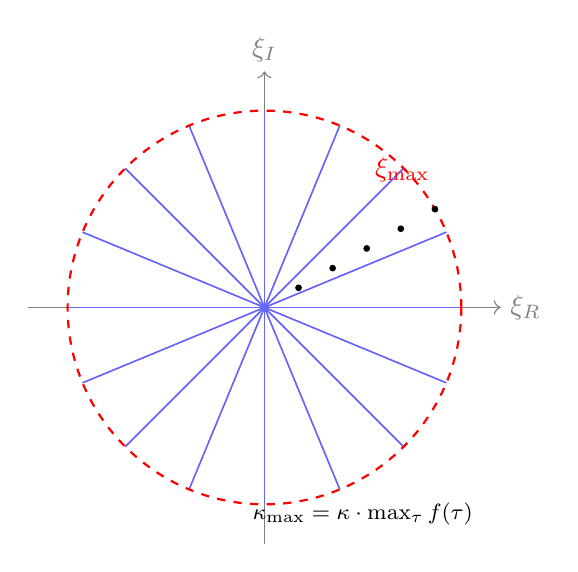
\begin{tikzpicture}[scale=2.5]
    % Coordinate axes
    \draw[->, gray] (-1.2,0) -- (1.2,0) node[right] {$\xi_R$};
    \draw[->, gray] (0,-1.2) -- (0,1.2) node[above] {$\xi_I$};

    % Radial spokes for different tau
    \foreach \angle in {0, 22.5, 45, 67.5, 90, 112.5, 135, 157.5, 180, 202.5, 225, 247.5, 270, 292.5, 315, 337.5} {
        \draw[blue!60, line width=0.5pt] (0,0) -- ({cos(\angle)}, {sin(\angle)});
        \draw[blue!60, line width=0.5pt] (0,0) -- ({-cos(\angle)}, {-sin(\angle)});
    }

    % Effective radius circle
    \draw[red, thick, dashed] (0,0) circle (1.0);
    \node[red] at (0.7, 0.7) {$\xi_{\max}$};

    % Sampling points on one spoke
    \foreach \r in {0.2, 0.4, 0.6, 0.8, 1.0} {
        \filldraw ({\r*cos(30)}, {\r*sin(30)}) circle (0.4pt);
    }

    % Annotation
    \node[font=\footnotesize] at (0.5, -1.05) {$\kappa_{\max} = \kappa \cdot \max_\tau f(\tau)$};
\end{tikzpicture}
\caption{Fourier 空间采样模式：不同 $\tau$ 对应不同方向的辐线（蓝色），
每条辐线上 $\omega_k$ 从 $0$ 到 $\omega_k^{\max}$ 采样（红圈内）。}
\label{fig:coverage}
\end{figure}

\begin{designbox}
\textbf{采样完备条件：} 要无失真的 2D 重建，需要 Nyquist 密度在傅里叶空间中满足
$\Delta\xi \lesssim \pi / \alpha_{\max}$。对于 $\alpha_{\max} = 8$（覆盖 BSV r=4 的
$|\alpha| \approx 4$ 反 squeezing），需要 $\Delta\xi \lesssim 0.4$。以 $N_\xi=128$、
$\xi_{\max}=19$ 为例，$\Delta\xi = 38/128 \approx 0.30$，满足要求。
\end{designbox}

% ======================================================================
\section{正则化策略}

\subsection{截断正则化（默认）}

最简单的正则化：在 $\omega_k^{\max}$ 处硬截断。参数由 SNR 公式自动确定，用户也可手动覆盖。

优点：无额外参数，物理意义清晰。缺点：硬截断在 $\alpha$ 空间产生 Gibbs 振铃。

\subsection{Tikhonov 正则化}

将硬截断替换为平滑衰减：
\[
\hat{Q}_{\text{reg}}(\boldsymbol{\xi}) = \frac{\hat{Q}(\boldsymbol{\xi})}
{1 + \lambda |\boldsymbol{\xi}|^2}
\]

$\lambda$ 控制阻尼强度。$\lambda \to 0$ 恢复无正则化；$\lambda \to \infty$ 仅保留直流分量。

\subsection{自适应策略}

首版实现采用截断正则化（零额外参数）。后续根据 closed-loop 测试结果决定是否需要
更复杂的正则化。

\begin{warnbox}
\textbf{不要过早优化正则化。} 在 closed-loop 测试通过之前，正则化的调优是无本之木。
先验证无噪声理想数据的反演精度，确认算法正确性后再逐步加入噪声和正则化。
\end{warnbox}

% ======================================================================
\section{验证方案}

\subsection{Closed-Loop 测试（Level 1 —— 算法正确性）}

\textbf{目标：} 验证反演算法在无近似误差、无噪声的理想条件下能否精确恢复 Q。

\begin{enumerate}
    \item \textbf{生成参考 Q}：选择一个解析 $Q$ 分布（如 BSV 的 Husimi-Q、双高斯混合等）
    \item \textbf{正向合成 P}：在连续极限下用解析核函数计算 $P(k,\tau)$：
        \[
        P(k_m,\tau_j) = \sum_{p,q} Q(\alpha_R[p],\alpha_I[q])\,
        \frac{1}{\sqrt{2\pi}\sigma_k}
        \exp\!\left[-\frac{(k_m - k_0 + \boldsymbol{\kappa}(\tau_j)\!\cdot\!\boldsymbol{\alpha}_{pq})^2}
        {2\sigma_k^2}\right] \Delta\alpha_R\Delta\alpha_I
        \]
    \item \textbf{反演}：对合成的 $P$ 执行完整反演流程
    \item \textbf{对比}：计算 $L_2$ 误差 $E = \|Q_{\text{recon}} - Q_{\text{ref}}\|_2 /
        \|Q_{\text{ref}}\|_2$，目视检查 2D 图
\end{enumerate}

\textbf{通过标准：} $L_2$ 误差 $< 1\%$，Q 的峰位置偏差 $< \Delta\alpha/2$。

\subsection{v5.1 对接测试（Level 2 —— 端到端）}

\textbf{目标：} 用 v5.1 完整 TDSE 正向模拟（含所有物理近似）的输出作为反演输入。

\begin{enumerate}
    \item 在 v5.1 中跑一个已知 Q 分布（如单相干态、BSV）的完整正向计算
    \item 将输出的 $P(k,\tau)$ 送入反演
    \item 对比反演 Q 和输入 Q
\end{enumerate}

\textbf{目的：} 量化 SFA、对角近似、离散化等实际近似对反演精度的综合影响。

\subsection{噪声鲁棒性测试（Level 3）}

对合成的 $P(k,\tau)$ 添加不同水平的 Poisson/Gaussian 噪声，测试反演稳定性。

% ======================================================================
\section{实现路线图}

\begin{table}[H]
\centering
\caption{实现阶段}
\begin{tabular}{p{1cm}p{3cm}p{4cm}p{4.5cm}}
\toprule
\textbf{阶段} & \textbf{名称} & \textbf{内容} & \textbf{产出} \\
\midrule
v1.0 & 最小可行 & 解析核正向 + 1D FFT + 截断 + 2D IFFT + closed-loop & 可运行脚本，验证算法 \\
\midrule
v1.1 & 数据对接  & 读取 v5.1 输出格式，预处理流水线 & 端到端可用 \\
\midrule
v1.2 & 正则化    & Tikhonov + TV 选项，噪声鲁棒性 & 实验数据可用 \\
\midrule
v2.0 & 迭代反演  & 考虑非对角项，交替估计 Q 和 $P_{\text{off}}$ & 高精度重建 \\
\bottomrule
\end{tabular}
\end{table}

\section{与 v5.1 正向模型的接口约定}

当 v5.1 用于为反演生成测试数据时，需遵循以下约定：

\begin{enumerate}
    \item $\tau$ 网格应均匀覆盖至少一个完整 NIR 周期
    \item $k$ 网格应均匀且包含 $k_0$ 的附近 ± $3\sigma_k$ 范围
    \item 输出需包含 $P(k,\theta,\phi;\tau)$ 的全部分波信息（对角和非对角分量分别保存）
        以便后续验证对角近似的影响
    \item 分支相位表需与振幅同步输出，供非对角项修正使用（v2.0+）
\end{enumerate}

% ======================================================================
\section{附录：关键公式速查}

\subsection{坐标约定}

\begin{itemize}
    \item $\alpha = \alpha_R + i\alpha_I$：相干态振幅（无量纲）
    \item $\boldsymbol{\alpha} = (\alpha_R, \alpha_I)^T$：实向量表示
    \item $\boldsymbol{\kappa}(\tau) = \kappa f(\tau)(\sin\omega\tau,\;\cos\omega\tau)^T$：
        streaking 向量
    \item $\boldsymbol{\xi} = (\xi_R, \xi_I)$：Fourier 空间坐标
    \item $k$：电子动量大小 (a.u.)
    \item $\tau$：XUV-NIR 延迟 (a.u.)
\end{itemize}

\subsection{默认物理常数（氢原子，800 nm NIR）}

\begin{table}[H]
\centering
\begin{tabular}{p{4cm}p{3cm}p{3cm}}
\toprule
\textbf{量} & \textbf{值} & \textbf{单位} \\
\midrule
$\omega$ (800 nm)  & 0.057   & a.u. \\
$T_{\text{NIR}}$   & 110.3   & a.u. (2.67 fs) \\
$\mathcal{E}_N$ ($10^{14}$ W/cm$^2$) & 0.04 & a.u. \\
$\kappa = 2\mathcal{E}_N/\omega$ & 1.4 & a.u. \\
$I_p$ (H 1s) & 0.5 & a.u. \\
$\Omega_{\text{XUV}}$ (典型) & 1.5--3.0 & a.u. (40--80 eV) \\
$k_0 = \sqrt{2(\Omega_{\text{XUV}}-I_p)}$ & 1.4--2.2 & a.u. \\
$\sigma_k \approx 1/\tau_X$ (200 as) & $\sim 0.2$ & a.u. \\
\bottomrule
\end{tabular}
\end{table}

\end{document}
